\documentclass[]{scrreprt}
\usepackage{amsmath,amsfonts,graphicx}
\usepackage{multirow}
\usepackage{pslatex}
\usepackage{tabularx}
\usepackage{comment}
\usepackage{xspace}
\usepackage{array}

\usepackage{hyperref}

\usepackage{caption}
\DeclareCaptionFont{white}{\color{white}}
\DeclareCaptionFormat{listing}{\colorbox{gray}{\parbox{\textwidth}{#1#2#3}}}

\graphicspath{
{figures/}
}

\newcommand{\uo}{\mbox{UO\textsubscript{2}}\xspace}

\setcounter{secnumdepth}{3}


\begin{document}


\title{Quick Two Phase (Q2P) Manual}
\author{Andy Wilkins \\
CSIRO}
\maketitle

\tableofcontents

%%%
\chapter{Introduction}
%%%

Quick Two Phase (Q2P) is a efficient and inflexible specialisation of
the Richards' equation.  It is designed to be ``quick'' to write input
files, and ``quick'' to run.
\begin{enumerate}
\item Q2P is only valid for 2-phases.
\item The capillary suction is somewhat obscured in Q2P compared with
  the Richards' formulation.  However, this is one of the keys behind
  Q2P's efficiency.  Often the true form of the capillary suction
  function is unknown in simulations of real-life materials.
\item Q2P is mass-lumped and fully-upwind only, with no options to
  make it otherwise
\end{enumerate}



%%%
\chapter{Theory and MOOSE implementation}
\label{chap.theory}
%%%


\section{DEs}

Call one phase ``water'', and denote it by the subscript $w$.  Call the
other phase ``gas'', and denote it by the subscript $g$.  The
variables of the system are the saturation of water, $S_{w}$, and the
porepressure of gas $P_{g}$.  The 2-phase Richards' equations are
\begin{eqnarray}
\phi \frac{\partial}{\partial t} \left( \rho_{w} S_{w} \right) & = & \nabla_{i}
\left( \frac{\rho_{w} \kappa_{ij}\kappa_{w}^{\mathrm{rel}}}{\mu_{w}} (\nabla_{j}P_{w} - \rho_{w} g_{j}) \right)
+ F_{w} \ , \nonumber \\
\phi \frac{\partial}{\partial t} \left( \rho_{g} S_{g} \right) & = & \nabla_{i}
\left( \frac{\rho_{g} \kappa_{ij}\kappa_{g}^{\mathrm{rel}}}{\mu_{g}} (\nabla_{j}P_{g} - \rho_{g} g_{j}) \right)
+ F_{w} \ .
\label{q2p_orig.eqn}
\end{eqnarray}
Please see the Richards' Theory Manual for a description of the
notation.

By capillarity $P_{w} = P_{g} - P_{c}(S_{w})$, and writing in terms of
the Q2P variables Eqn~(\ref{q2p_orig.eqn}) reads
\begin{eqnarray}
\phi \frac{\partial}{\partial t} \left( \rho_{w} S_{w} \right) - \nabla_{i}
\left( \frac{\rho_{w} \kappa_{ij}\kappa_{w}^{\mathrm{rel}}}{\mu}
(\nabla_{j}P_{g} - \rho_{w} g_{j}) \right) - \nabla_{i}\left(
\frac{\rho_{w}\kappa_{ij}D}{\mu_{w}} \nabla S_{w} \right)
- F_{w} & = & 0 \ \ \ \mbox{[variable $S_{w}$]}\ \ , \nonumber \\
\phi \frac{\partial}{\partial t} \left( \rho_{g} (1 - S_{w}) \right) - \nabla_{i}
\left( \frac{\rho_{g} \kappa_{ij}\kappa_{g}^{\mathrm{rel}}}{\mu} (\nabla_{j}P_{g} - \rho_{g} g_{j}) \right)
- F_{g} & = & 0 \ \ \ \mbox{[variable $P_{g}$]}\ \ .
\label{q2p.eqn}
\end{eqnarray}
The main step here has been to define the diffusivity
\begin{equation}
D(S_{w}) = -\kappa_{w}(S_{w})P_{c}'(S_{w}) \geq 0 \ ,
\end{equation}
but also it is assumed that
\begin{eqnarray}
\rho_{w} & = & \rho_{w}(P_{g}) \ , \nonumber \\
\rho_{g} & = & \rho_{g}(P_{g}) \ , \nonumber \\
\kappa_{w}^{\mathrm{rel}} & = & \kappa_{w}^{\mathrm{rel}}(S_{w}) \ ,
\nonumber \\
\kappa_{g}^{\mathrm{rel}} & = & \kappa_{g}^{\mathrm{rel}}(S_{w}) \ .
\end{eqnarray}
Hence Eqn~(\ref{q2p.eqn}) is two equations in two unknowns $S_{w}$ and
$P_{g}$.

Often $\rho_{w}$ is almost constant compared with the range of $P_{g}$
in the problems, so that the first of Eqn~(\ref{q2p.eqn}) looks very
similar to a diffusion equation with diffusivity $D$.  In the Q2P
module it is assumed that
\begin{equation}
D = \tilde{D}\tilde{\kappa}^{\mathrm{rel}}_{w}(S_{w})
\ ,
\label{diffusivity.eqn}
\end{equation}
where $\tilde{D}$ is a {\em constant} and $\tilde{\kappa}$ defaults to
be the water relative permeability function, but may be set to another
relative permeability curve (eg, a constant), if desired.
Hence the capillary suction is rather obscured,
although $D$ is directly proportional to $P_{c}$ and has the same
units as it.  The Q2P module can handle very small $D$ (ie, very small
$P_{c}$) more efficiently than the full Richards module.  However,
setting $D=0$ leads to shocks forming in most problems so it is not
recommended.


\section{Actions}

The {\tt Q2P} action includes all the Q2P Kernels below, as well as,
optionally, nodal mass AuxVariables and total fluid mass
Postprocessors for mass-balance calculations.

\section{Kernels}

Eqn~(\ref{q2p.eqn}) has five terms (along with the source terms) which
are encoded in the following kernels.

\begin{itemize}

\item {\tt Q2PNodalMass} encodes both $\phi \rho_{w}
  S_{w}/{\mathrm{d}}t$ and $\phi \rho_{g} (1 - S_{w})/{\mathrm{d}}t$.
  It is lumped to the nodes.  It is designed to work with the {\tt
    Q2PNegativeNodalMassOld} in order to form the time derivative of
  the fluid masses.  This Kernel requires:
\begin{itemize}
\item A Material that defines ``porosity''.
\item The user to define ``fluid\_density'' which is a RichardsDensity
  UserObject that defines $\rho$ as a function of $P_{g}$.
\item The names of the Variables $S_{w}$ and $P_{g}$.
\item Whether the Variable is porepressure.  This latter flag should
  be false for the water equation, and true for the gas equation.
\end{itemize}

\item {\tt Q2PNegativeNodalMassOld} encodes the old values of both
  $-\phi \rho_{w} S_{w}/{\mathrm{d}}t$ and $-\phi \rho_{g} (1 -
  S_{w})/{\mathrm{d}}t$.  It is lumped to the nodes.  It is designed
  to work with the {\tt Q2PNodalMass} in order to form the
  time derivative of the fluid masses.  This Kernel requires:
\begin{itemize}
\item A Material that defines ``porosity''.
\item The user to define ``fluid\_density'' which is a RichardsDensity
  UserObject that defines $\rho$ as a function of $P_{g}$.
\item The names of the Variables $S_{w}$ and $P_{g}$.
\item Whether the Variable is porepressure.  This latter flag should
  be false for the water equation, and true for the gas equation.
\end{itemize}

\item {\tt Q2PSaturationFlux} encodes $ - \nabla_{i}
\left( \frac{\rho_{w} \kappa_{ij}\kappa_{w}^{\mathrm{rel}}}{\mu}
(\nabla_{j}P_{g} - \rho_{w} g_{j}) \right)$.  It is fully upwinded.
This Kernel requires:
\begin{itemize}
\item The Variable to be $S_{w}$.
\item A Material that defines ``gravity'' and ``permeability''.
\item The name of the $P_{g}$ variable.
\item The fluid dynamic viscosity $\mu_{w}$.
\item The ``fluid\_density'' which is a RichardsDensity
  UserObject that defines $\rho_{w}$ as a function of $P_{g}$.
\item The ``fluid\_relperm'' which is a RichardsRelPerm UserObject that
  defines the fluid relative permeability as a function of the $S_{w}$
  variable.  For instance this UserObject could have type
  RichardsRelPermPower.
\end{itemize}

\item {\tt Q2PPorepressureFlux} encodes $ - \nabla_{i}
\left( \frac{\rho_{g} \kappa_{ij}\kappa_{g}^{\mathrm{rel}}}{\mu}
(\nabla_{j}P_{g} - \rho_{g} g_{j}) \right)$.  It is fully upwinded.
This Kernel requires:
\begin{itemize}
\item The Variable to be $P_{g}$.
\item A Material that defines ``gravity'' and ``permeability''.
\item The name of the $S_{w}$ variable.
\item The fluid dynamic viscosity $\mu_{g}$.
\item The ``fluid\_density'' which is a RichardsDensity
  UserObject that defines $\rho_{g}$ as a function of $P_{g}$.
\item The ``fluid\_relperm'' which is a RichardsRelPerm UserObject that
  defines the fluid relative permeability as a function of the $S_{w}$
  variable.  {\em Note} this could be a Q2PRelPermPowerGas UserObject,
  and {\em not} a RichardsRelPermPower UserObject since it must be a
  function of $S_{w}$ and {\em} not $S_{g}$.
\end{itemize}

\item {\tt Q2PSaturationDiffusion} encodes $- \nabla_{i}\left(
\frac{\rho_{w}\kappa_{ij}D}{\mu_{w}} \nabla S_{w} \right)$.  It is not
upwinded.  This Kernel requires:
\begin{itemize}
\item The Variable to be $S_{w}$.
\item A Material that defines ``permeability''.
\item The name of the porepressure variable
\item The ``fluid\_density'' which is a RichardsDensity
  UserObject that defines $\rho_{w}$ as a function of $P_{g}$.
\item The fluid dynamic viscosity $\mu_{w}$.
\item The diffusivity constant $\tilde{D}$.
\item the ``fluid\_relperm'' which is a RichardsRelPerm UserObject
  that defines the diffusivity as per Eqn~(\ref{diffusivity.eqn}).
\end{itemize}

\end{itemize}


\section{Other classes}

\subsection{Relative permeability}

For the water phase, all the ``RichardsRelPerm'' objects may be
used, as they are all functions of $S_{w}$.  However, for the gas
phase, these shouldn't be used.  Instead the ``Q2PRelPerm'' objects
should be used.  These are:

\begin{itemize}
\item {\tt Q2PRelPermPowerGas}.  Define $S = S_{w}/(1 -
  S_{\mathrm{imm}})$, where $S_{\mathrm{imm}}$ is the immobile
  saturation of the gas.  The relative permeability is
\begin{equation}
\kappa_{g}^{\mathrm{rel}} = \left\{
\begin{tabular}{ll}
1 & \mbox{ for } $S_{w} \leq 0$ \\
$1 - (n+1)S^{n} + nS^{n+1}$ & \mbox{ for } $0 < S_{w} < 1 -
S_{\mathrm{imm}}$ \\
0 & \mbox{ for } $S_{w} \geq 1 - S_{\mathrm{imm}}$ \\
\end{tabular}
\right.
\end{equation}

\end{itemize}


\subsection{Materials}

The ``Q2PMaterial'' is a vastly stripped-down version of
``RichardsMaterial''.  It provides porosity, permeability and gravity
only.  No mobility, SUPG, etc, calculations are needed, which can
enhance compute speed substantially over a similar Richards
simulation.



\subsection{DiracKernels}

The ``Q2PBorehole'' behaves in a similar way to a
``RichardsBorehole'' but correctly calculates the Jacobian entries in
the Q2P setting.



\subsection{BCs}

The ``Q2PPiecewiseLinearSink'' behaves in a similar way to the
``RichardsPiecewiseLinearSink'' but correctly calculates the Jacobian
entries in the Q2P setting.


\subsection{Postprocessors}

The ``Q2PPiecewiseLinearSinkFlux'' records the water or gas mass flow
into a Q2PPiecewiseLinearSink, in the same way as
RichardsPiecewiseLinearSinkFlux.



%%%
\chapter{Tests}
%%%

\section{Jacobians}

The Jacobian of all the Kernels, DiracKernels and BCs are tested.

\section{Hydrostatic head}

It is demonstrated that Q2P's steady-state is hydrostatic head as
expected (the test is called gravity\_head\_2.ghQ2P\_pgas).

\section{Q2PBorehole}

The flow rates of gas and water into a production borehole are tested
(in test dirac.q2p01)
and found to be in agreement with expectations as shown in
Figure~\ref{bh.fig}.  At the same time, mass conservation is tested.

\begin{figure}[htb]
\centering
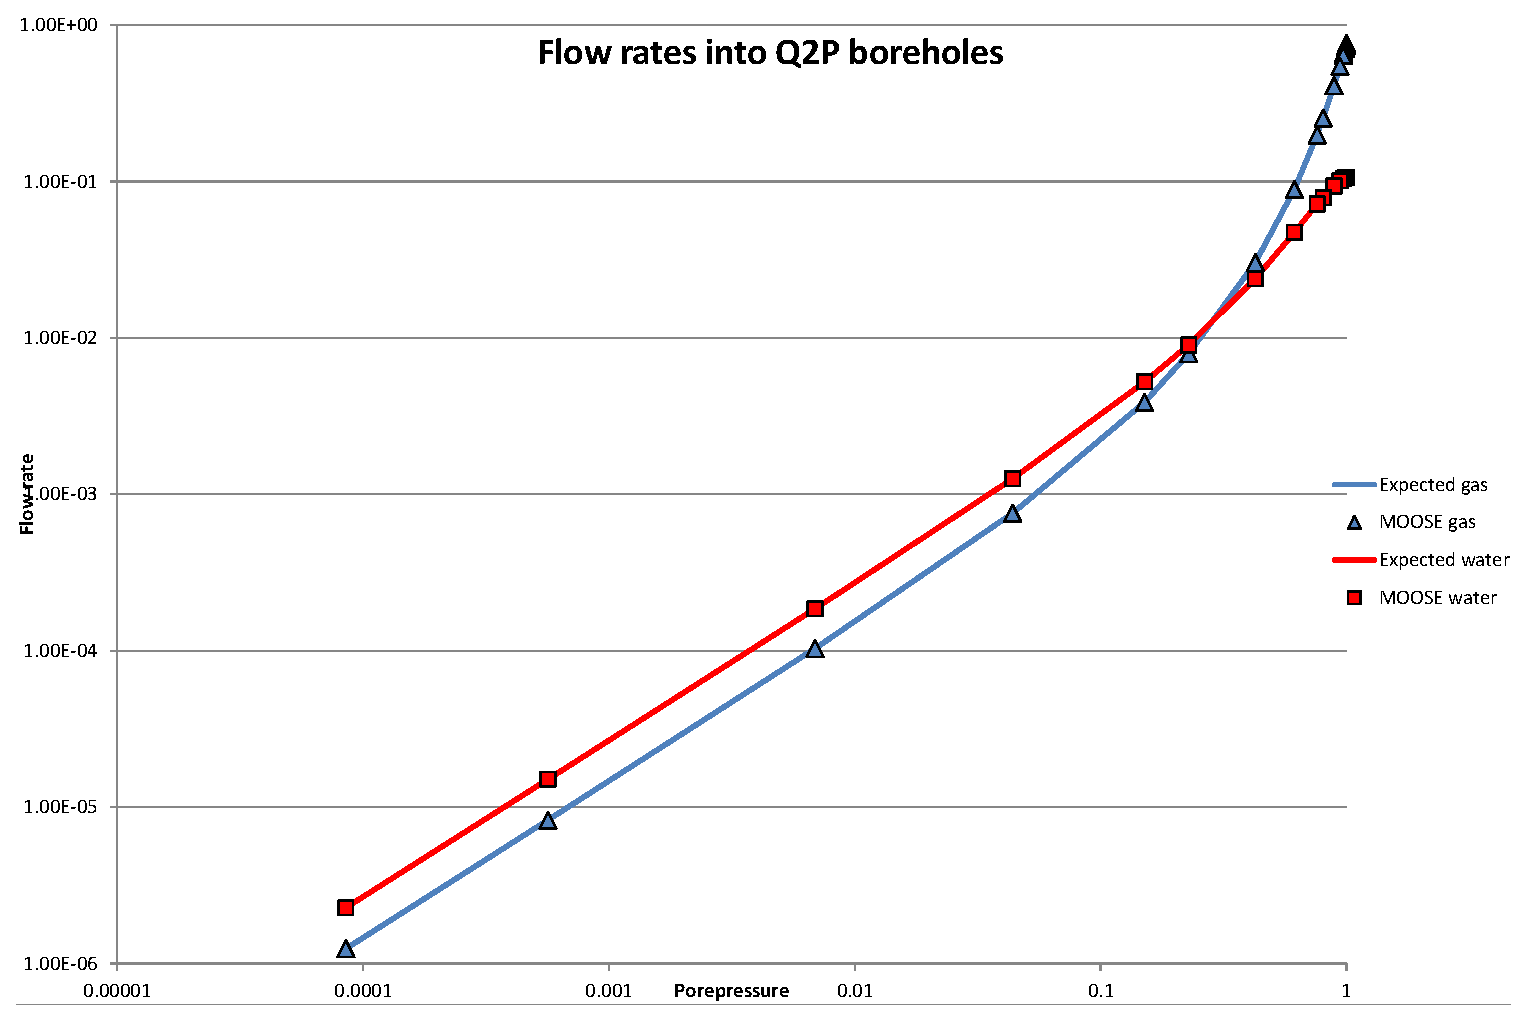
\includegraphics[width=8cm]{bh.eps}
\caption{Gas and water flow rates into a production borehole.  The
  MOOSE implementation agrees with the expected results.}
\label{bh.fig}
\end{figure}

\section{Q2PPiecewiseLinearSink}

The flow rates from Q2PPiecewiseLinearSink, and those recorded by
Q2PPiecewiseLinearSinkFlux, are tested in sinks.q2p01.  Mass balances
are shown to be correct.  Fluxes of water and gas with and without
relative permeability and density contributions are shown to be as
expected.  See an example in Figure~\ref{q2p01_sink.fig}.

\begin{figure}[htb]
\centering
\includegraphics[width=8cm]{q2p01_sink.eps}
\caption{Flux into a Q2PPiecewiseLinearSink as calculated by one of
  the sinks in sinks.q2p01.  The
  MOOSE implementation agrees with the expected results.}
\label{q2p01_sink.fig}
\end{figure}





%%%
\chapter{Comments for users}
%%%

The Richards theory, test and user manual all contain pertinant
information for the user on convergence criteria, tips for ensuring
and speeding convergence, etc.  The following points pertain
specifically to the Q2P formulation.

\begin{enumerate}
\item Setting the diffusivity can be key to ensuring good convergence.
  If it is set too small then shocks will form.  If you observe this
  occuring, eg, the saturation   varies from 0 to 1 over one element,
  then $D$ should be increased.

\item I have found the system can exit the physical region $0\leq
  S_{w} \leq 1$ more easily than in the Richards formulation.  I'm not
  sure why this occurs.  I have found that setting nonzero immobile
  saturations prevents this (and nonzero immobile saturations are
  correct physically anyway).

\item Because two densities treat the gas and water pressures are
  identical, the water density must be zero at zero pressure.  In the
  Richards formulation this is not the case, as water density can be
  positive even for negative water pressure.  However, in the Q2P
  situation, if the water pressure is negative then so too is the gas
  pressure, and in this case the gas density would be undefined.
  Therefore Q2P requires $P_{g}\geq 0$.  To ensure this, the water
  density must satisfy $\lim_{P\rightarrow 0}\rho_{w}(P) = 0$.  An
  example is {\tt RichardsDensityConstbulkCut}.

\end{enumerate}






\end{document}

